
\medskip
L'ISS (International Space Station) est une station spatiale internationale placée en orbite autour de la Terre.

\begin{enumerate}
	\item Dans la journée du 21 juin 2021, l’ISS est passée à la verticale de Canberra (Australie) puis à la verticale de Miami (Etats-Unis).

À l'aide du planisphère ci-dessous, donner les coordonnées géographiques de ces deux villes avec la précision permise par le graphique.
\end{enumerate}
\begin{center}
		\begin{tikzpicture}[scale=0.85]
		\node at (-8,-4.2) {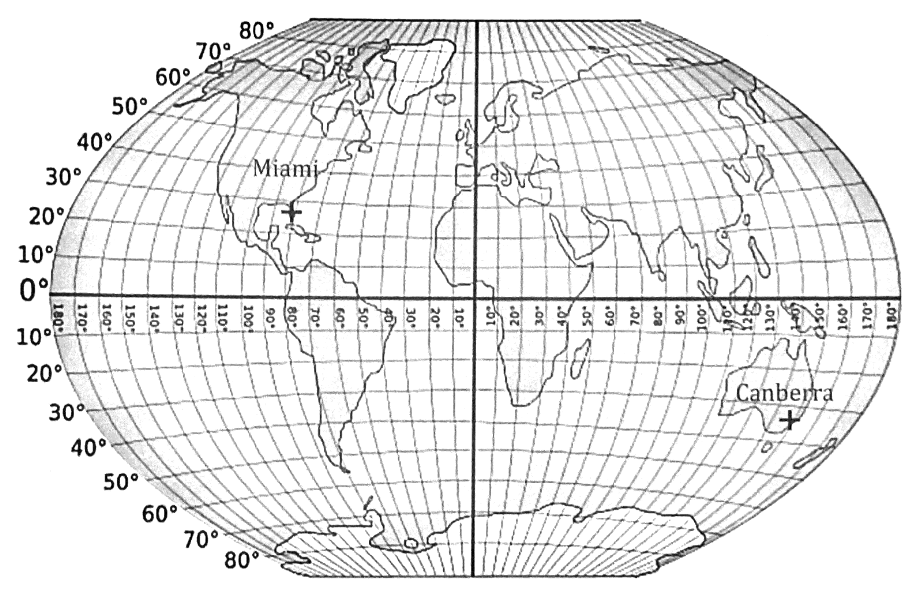
\includegraphics{planisphere.eps}};
		\draw
			(0:1) node[right]{E} --
			(45:0.2) --
			(90:1) node[above]{N} --
			(135:0.2)--
			(180:1) node[left]{O} --
			(215:0.2) --
			(-90:1) node[below]{S} --
			(-45:0.2) -- cycle;
			\foreach \a in {0,90,180,270}
				\fill[fill=black] (0,0)--(\a:1)--(\a+45:.2)--cycle;

	\end{tikzpicture}

\end{center}

On représente la Terre, l'ISS et son orbite (trajectoire de l’ISS) à l'aide du schéma ci-dessous.

\medskip

\begin{minipage}{8cm}
	On considère que:
\begin{itemize}
	\item la Terre est assimilée a une sphère de rayon \np[km]{6371};

	\item l’orbite de l’ISS est un cercle de même centre que celui de la Terre ;

	\item l’ISS tourne autour de la Terre a une altitude de $380$ km.
\end{itemize}
\end{minipage}
\hfill
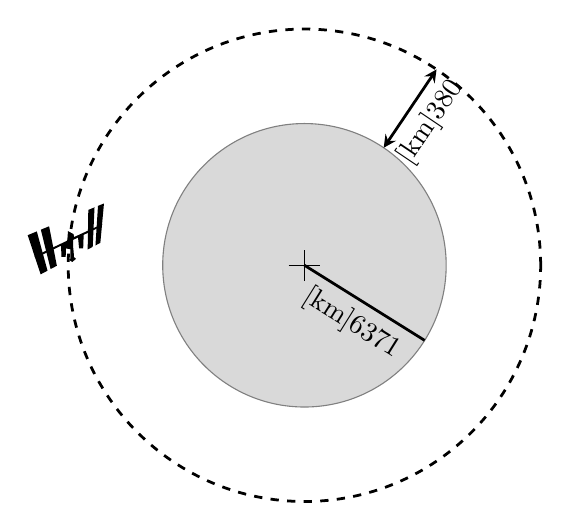
\begin{tikzpicture}[baseline={(0,0)}]
	\draw[draw = gray,fill=gray!30] (0,0) circle (1.8);
	\draw (-0.2,0)--(0.2,0) (0,-0.2)--(0,0.2);
	\draw[line width=1 pt, dashed] (0,0) circle (3);
	\draw [line width = 1pt , <->,> = stealth]
		(0,0)--(-32:1.8) node [pos=.5,below,sloped] {\np[km]{6371}}
		(56:1.8)--(56:3) node [pos=.5,below,sloped] {\np[km]{380}};

		\fill[line width=0.8pt,fill=black,shift={(0,0)}] (-3.515,0.382) -- (-3.399,0.430) -- (-3.263,-0.069) -- (-3.350,-0.115) -- cycle;
		\fill[line width=0.8pt,fill=black,shift={(0,0)}] (-3.348,0.452) -- (-3.243,0.495) -- (-3.144,-0.006) -- (-3.224,-0.048) -- cycle;
		\fill[line width=0.8pt,fill=black,shift={(0,0)}] (-2.745,0.703) -- (-2.666,0.736) -- (-2.689,0.234) -- (-2.753,0.200) -- cycle;
		\fill[line width=0.8pt,fill=black,shift={(0,0)}] (-2.622,0.754) -- (-2.546,0.785) -- (-2.592,0.285) -- (-2.654,0.252) -- cycle;
		\fill[line width=0.8pt,fill=black,shift={(0,0)}] (-3.427,0.116) -- (-3.020,0.309) -- (-3.011,0.325) -- (-3.003,0.434) -- (-2.932,0.395) -- (-2.927,0.358) -- (-2.570,0.522) -- (-2.573,0.497) -- (-2.804,0.386) -- (-2.810,0.215) -- (-2.862,0.215) -- (-2.875,0.352) -- (-2.937,0.323) -- (-2.937,0.224) -- (-2.930,0.164) -- (-2.929,0.106) -- (-2.901,0.082) -- (-2.948,0.042) -- (-2.990,0.068) -- (-2.973,0.083) -- (-2.974,0.204) -- (-2.990,0.207) -- (-3.029,0.214) -- (-3.032,0.106) -- (-3.086,0.108) -- (-3.091,0.248) -- (-3.418,0.091) -- cycle;
\end{tikzpicture}

\begin{enumerate}[resume]
	\item Montrer que l’ISS parcourt environ \np[km]{42400} pour effectuer un tour complet de la Terre.

	\item On estime que l’ISS tourne autour de la Terre à la vitesse moyenne de \np[km/h]{27600}.
	\begin{enumerate}
		\item Montrer qu’il faut environ 1~h~32~min à l'ISS pour effectuer un tour complet de la Terre.
		\item Le 19 juin 2020, de 14~h~30 à 21~h~45 (heure de Paris), le spationaute français Thomas Pesquet a effectué une sortie extravéhiculaire en restant attaché à |’ISS.

		Durant cette sortie, combien de fois Thomas Pesquet a-t-il fait le tour complet de la Terre ?
	\end{enumerate}
\end{enumerate}
